\section{Introduction}

LLM-based agents~\citep{DBLP:journals/fcsc/WangMFZYZCTCLZWW24} are increasingly deployed in real-world scenarios, where they must move beyond instantaneous problem-solving toward long-term proficiency~\citep{he2026memoryarena}. However, the prevailing paradigm of ``one-off'' task execution limits their utility in streaming settings, where tasks unfold sequentially over time. This makes \emph{self-evolution}~\citep{fang2025comprehensive, gao2025survey} essential: capable agents should not repeatedly start from scratch, but instead continually accumulate, refine, and reuse experience for future tasks.

A key substrate for self-evolution is \emph{procedural memory}~\citep{hu2025memory, wu2025human, DBLP:journals/corr/abs-2508-06433}, specifically, reusable skills~\citep{anthropic_skills_2025, wang2025inducing} accumulated from past interactions. In real-world streaming settings~\citep{wu2024streambench}, a skill-based self-evolving agent typically follows a closed-loop workflow: for each new task, it selects relevant skills, uses them to guide execution, and updates its skill collection based on the resulting trajectory. This makes skill curation---the extraction of high-quality lessons and their integration into the skill collection---essential for self-evolving agents.

However, existing skill curation works remain limited. Manually curated skills, such as Anthropic's skills repository~\citep{anthropic_skills_2025}, demand huge human expertise and cannot scale to the diversity of tasks that agents may encounter. Prompting or heuristic-based methods that dictate memory operations~\citep{xu2025amem, qiu2025alita, DBLP:journals/corr/abs-2504-07079} rely on fixed rules and lack downstream performance feedback, preventing them from adapting to the executor's actual needs. Recent studies explored reinforcement learning (RL) to optimize skill-based agent systems. However, they either focus on teaching agents to \textit{use} skills~\citep{xia2026skillrl, tu2026dynamic} or
optimize skill operations within a short task stream~\citep{DBLP:journals/corr/abs-2512-17102, DBLP:journals/corr/abs-2602-10652}. This limits the density of learning signals available for curating highly reusable skills and mastering complex management operations such as skill update and deletion, which are essential for robust and scalable long-term self-evolution.

\begin{figure}[t]
\begin{center}
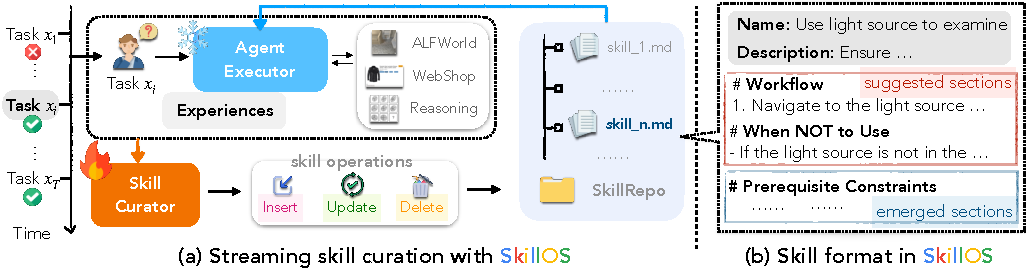
\includegraphics[width=0.98\textwidth]{figures/SkillOS_workflow.pdf}
\end{center}
\vspace{-3mm}
\caption{\ours{} pairs a frozen \textit{Agent Executor} with a trainable \textit{Skill Curator}. The executor retrieves relevant skills from \textsc{SkillRepo} to act; the curator edits the repo (insert/update/delete) based on the resulting experiences, with Markdown as the skill format.
}
\label{fig: skillos_overview}
\vspace{-5mm}
\end{figure}

To tackle this challenge, we propose\skillos, an experience-driven RL training recipe to learn the capability of skill curation for self-evolving agents. 
We study skill curation in a modular multi-agent framework in a streaming setting, where a frozen \emph{agent executor} solves tasks with a skill collection (termed \textsc{SkillRepo}), while a trainable \emph{skill curator} updates and manages this collection through function calls (Figure~\ref{fig: skillos_overview}\textcolor{redlinkcolor}{(a)}).
We represent skills as Markdown files~\citep{anthropic_skills_2025} (Figure~\ref{fig: skillos_overview}\textcolor{redlinkcolor}{(b)}) managed via file I/O operations similar to an operating system (OS).
Our recipe features two core designs. 
\textit{First}, we construct each training instance as a group of related tasks. By mimicking test-time streaming settings, it grounds skill curation in long-term utility: skills induced from earlier experiences are evaluated by their ability to improve later related tasks.
\textit{Second}, we design rewards to better attribute environmental feedback to curation decisions, combining task performance with signals for valid function calls, skill quality, and \textsc{SkillRepo}'s compactness. Together, these designs turn delayed and indirect supervision into learning signals for skill curation.

We evaluate \ours{} on both multi-turn agentic tasks and single-turn reasoning tasks. Experiments show that \ours{} consistently outperforms memory-free and strong memory-based methods in both effectiveness and efficiency, with up to $+9.8\%$ relative performance improvement and $-6.0\%$ fewer interaction steps compared to the strongest baseline (Table~\ref{table: alfworld}). Our trained skill curator generalizes well across executors and tasks, improving performance even with the Gemini-2.5-Pro executor. Notably, our 8B curator also outperforms Gemini-2.5-Pro when used directly as the curator. Beyond performance gains, our analyses further show that the learned skill curator leads to more targeted and effective skill utilization, while the skills in \textsc{SkillRepo} evolve into more richly structured Markdown files that encode higher-level meta-skills over time. Together, we establish \ours{} as a practical, modular, and experience-driven RL training recipe for building self-evolving agents.